\chapter{Schiere di antenne}

	Vedremo in questo capitolo come combinare in modo opportuno una serie di antenne per migliorare le prestazioni del nostro ricevitore.

\section{Schiera di antenne isotrope}
	Il caso più semplice è quello di una serie lineare ed equispaziata di antenne isotrope, ovvero antenne che irradiano in modo uniforme in tutte le direzioni.

	Esse sono un utile astrazione, perché ci permettono di considerare le proprietà del posizionamento delle antenne indipendentemente dalle loro particolarità.

	\begin{figure}[ht]
		\centering
		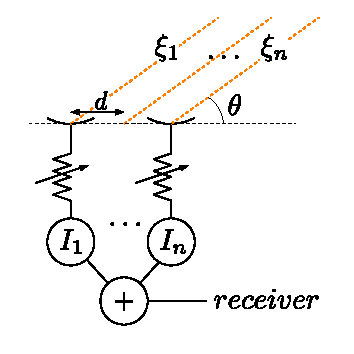
\includegraphics{img/schiera_antenne.pdf}
		\caption{Le antenne della schiera sono alimentate dalle correnti $I_i$ e ricevono il segnale dal campo lontano con sfasamenti diversi $\xi_i$.}
		\label{fig:schiera}
	\end{figure}

	Dallo schema elettrico in figura \ref{fig:schiera} si può facilmente calcolare il segnale in arrivo al ricevitore, definito come \gls{af}.

	\begin{esp} \label{eq:array_factor}
		AF = \sum_{i=1}^n I_i e^{\jmath \xi_i}
			\stackrel{(*)}{=} \sum_{i=1}^n I_i ~ e^{\jmath (i-1) \beta d \cos \theta}
	\end{esp}
	dove in (*) si calcola la differenza di cammino tra i vari percorsi.

	D'ora in avanti considereremo sempre alimentazioni $I_i$ sfasate tra loro di un angolo $\alpha$ costante: in questo caso il calcolo dell'\gls{af} si riduce a

	\begin{esp}
		AF = \sum_{i=1}^n A_i ~ e^{\jmath (i-1) (\beta d \cos \theta + \alpha)}
			\stackrel{.}{=} \sum_{i=1}^n A_i ~ e^{\jmath (i-1) \psi}
	\end{esp}
	dove $I_i$ viene scomposto in modulo e fase come $A_i ~ e^{\jmath (i-1) \alpha}$ e $\psi$ è detto
